
\begin{table*}[ht]
    \caption{Scores achieved on the Proprio Control 50/100k and Vision Control 100/200k benchmarks (with 3 seeds run for each) demonstrate that EZ-V2 consistently maintains sample efficiency, whether with proprioceptive or visual inputs. The tasks are categorized into easy and hard groups as proposed by \citep{hubert2021learning}. The results of DreamerV3 are sourced from the official data \citep{hafner2023mastering}.}
    \label{tab:dmc_results_full}
\begin{center}
\begin{small}
% \begin{sc}
\centering
\scalebox{0.85}{
\centering
\begin{tabular}{l|cccc|cccc}
\toprule
\multicolumn{1}{l|}{\large Benchmark} & \multicolumn{4}{c|}{\large Proprio Control 50k} & \multicolumn{4}{c}{\large Vision Control 100k} \\
\midrule
Task &   SAC &  TD-MPC2 &   DreamerV3 & \textbf{EZ-V2 (Ours)} &   CURL &  DrQ-v2 &    DreamerV3 & \textbf{EZ-V2 (Ours)}  \\
\midrule
Cartpole Balance             &      \textbf{997.6} &   \underline{962.8}&     839.6 &    947.3 &    \underline{963.3} &    \textbf{965.5} &   956.4 & 911.7  \\
Cartpole Balance Sparse             &    \underline{993.1} &    942.8 &    559.0 &   \textbf{999.2} &    \underline{999.4} &    \textbf{1000.0} &   813.0 & 951.5 \\
Cartpole Swingup            &    \textbf{861.6} &   \underline{826.7} &   527.7 &   805.4 &    \textbf{765.4} &    \underline{756.0} &   374.8 & 747.8  \\
Cup Catch              &      949.9 &    \textbf{976.0} &      729.6&     \underline{969.8} &      932.3&      468.0 &    \underline{947.7} & \textbf{954.7}  \\
Finger Spin            &      \underline{900.0} &     \textbf{965.8} &    765.8 &     837.1 &      \underline{850.2} &     459.4 &    633.2 & \textbf{927.6}  \\
Pendulum Swingup           &     158.9 &   520.1&    \textbf{830.4} &   \underline{825.4} &   144.1 &    233.3 &  \underline{619.3} &  \textbf{726.7}  \\
Reacher Easy           &     744.0 &    \underline{903.5} &    693.4 &   \textbf{940.3} &    467.9 &    \underline{722.1} &   441.4 & \textbf{946.3} \\
Reacher Hard           &     646.5 &   580.4 &    \underline{768.0} &   \textbf{795.4}  &    112.7 &    \underline{202.9} &  120.4 & \textbf{961.5} \\
Walker Stand      &   870.0 &  \textbf{973.9} &  767.3 &  \underline{953.6} &  733.8 &   426.1 & \underline{939.5} & \textbf{944.9}  \\
Walker Walk           &    813.2 &   \textbf{965.5} &   475.2 &   \underline{944.0} &   538.5 &   681.5 &  \underline{771.2} & \textbf{888.8}  \\
\midrule
\multicolumn{1}{l|}{} & \multicolumn{4}{c|}{\large Proprio Control 100k} & \multicolumn{4}{c}{\large Vision Control 200k} \\
\midrule
Acrobot Swingup               &    44.1 &   \textbf{303.2}&    62.8 &   \underline{297.7} &    6.8 &    15.1 &   \underline{67.4} & \textbf{231.8} \\
Cartpole Swingup Sparse         &     256.6 &    \underline{421.4} &     172.7 &   \textbf{795.4} &    8.8 &    81.2 &   \underline{392.4} & \textbf{763.6} \\
Cheetah Run          &   \textbf{680.9} &  614.4 &   400.8 &  \underline{677.8} &  405.1 &  418.4 & \underline{587.3} & \textbf{631.6}  \\
Finger Turn Easy           &    \underline{630.8} &   \textbf{793.3} &   560.5 &  310.7 & \underline{371.5} &    286.8 &   366.6 & \textbf{799.2}  \\
Finger Turn Hard      &  414.0 &  \textbf{604.8} &  \underline{474.2} & 374.1 &  236.3 &  \underline{268.4} & 258.5 & \textbf{794.6} \\
Hopper Hop        &    0.1 &   \underline{84.5} &    9.7 &   \textbf{186.5} &    \underline{84.5}&   26.3&   76.3 & \textbf{206.4} \\
Hopper Stand             &      3.8 &     \textbf{807.9} &     296.1 &    \underline{795.4} &     627.7 &      290.2 &    \underline{652.5} & \textbf{805.7} \\
Quadruped Run              &    139.7 &   \textbf{742.1} &   289.0  &   \underline{510.6} &    170.9 &    \underline{339.4} &   168.0 & \textbf{384.8}  \\
Quadruped Walk               &   237.5 & \underline{853.7} &   256.2 &  \textbf{925.8} &   131.8 &   \underline{311.6} &  122.6 & \textbf{433.3} \\
Walker Run              &   635.4 &   \textbf{780.5} &   478.9 &  \underline{657.2} &   274.7 &   359.9 &  \textbf{618.2} & \underline{475.3}\\
\midrule
\multicolumn{1}{l|}{Mean}         &    552.0 &    \textbf{740.9} &    517.1 &    \underline{723.2} &   437.3 &    410.3 &   \underline{498.5} & \textbf{726.1}  \\
\multicolumn{1}{l|}{Median}        &    633.3 &    \textbf{806.4} &    543.4 &    \underline{800.4} &   324.9 &    330.6 &  \underline{484.5} & \textbf{788.1}    \\

\bottomrule
%\vskip -0.5cm
\end{tabular}
}
\end{small}
\end{center}
\end{table*}

% \begin{table*}[ht]
%     \caption{Scores achieved on the Proprio Control 50/100k and Vision Control 100/200k benchmark (we run 3 seeds). EfficientZero-v2 achieves consistent sample efficiency with proprioceptive or visual inputs.}
%     \label{tab:dmc_results_full}
% \begin{center}
% \begin{small}
% % \begin{sc}
% \centering
% \scalebox{0.85}{
% \centering
% \begin{tabular}{ll|cccc|cccc}
% \toprule
% \multicolumn{2}{c|}{\large Benchmark} & \multicolumn{4}{c|}{\large Proprio Control 50k} & \multicolumn{4}{c}{\large Vision Control 100k} \\
% \midrule
% Level &Task &   SAC &  TD-MPC2 &   DreamerV3 & \textbf{EZ-V2 (Ours)}&   CURL &  DrQ-v2 &    DreamerV3 & \textbf{EZ-V2 (Ours)}& \\
% \midrule
% \multirow{11}{*}{\textbf{Easy}} & Cartpole Balance             &      \textbf{997.6} &   962.8&     839.6 &    947.3 &    \textbf{963.3} &    \textbf{965.5} &   956.4 & 911.7  \\
% & Cartpole Balance Sparse             &    993.1 &    942.8 &    559.0 &   \textbf{999.2} &    \textbf{999.4} &    \textbf{1000.0} &   813.0 & 951.5 \\
% & Cartpole Swingup            &    \textbf{861.6} &   826.7 &   527.7 &   805.4 &    \textbf{765.4} &    756.0 &   374.8 & 747.8  \\
% & Cup Catch              &      949.9 &    \textbf{976.0} &      729.6&     \textbf{969.8} &      932.3&      468.0 &    947.7 & \textbf{954.7}  \\
% & Finger Spin            &      900.0 &     \textbf{965.8} &    765.8 &     837.1 &      850.2 &     459.4 &    633.2 & \textbf{927.6}  \\
% & Pendulum Swingup           &     158.9 &   520.1&    \textbf{830.4} &   \textbf{825.4} &   144.1 &    233.3 &  619.3 &  \textbf{726.7}  \\
% & Reacher Easy           &     744.0 &    903.5 &    693.4 &   \textbf{940.3} &    467.9 &    722.1 &   441.4 & \textbf{946.3} \\
% & Reacher Hard           &     646.5 &   580.4 &    768.0 &   \textbf{795.4}  &    112.7 &    202.9 &  120.4 & \textbf{961.5} \\
% & Walker Stand      &   870.0 &  \textbf{973.9} &  767.3 &  953.6 &  733.8 &   426.1 & 939.5 & \textbf{944.9}  \\
% & Walker Walk           &    813.2 &   \textbf{965.5} &   475.2 &   944.0 &   538.5 &   681.5 &  771.2 & \textbf{888.8}  \\
% \midrule
% \multicolumn{2}{c|}{} & \multicolumn{4}{c|}{\large Proprio Control 100k} & \multicolumn{4}{c}{\large Vision Control 200k} \\
% \midrule
% \multirow{9}{*}{\textbf{Hard}} & Acrobot Swingup               &    44.1 &   \textbf{303.2}&    62.8 &   \textbf{297.7} &    6.8 &    15.1 &   67.4 & \textbf{231.8} \\
% & Cartpole Swingup Sparse         &     256.6 &    421.4 &     172.7 &   \textbf{795.4} &    8.8 &    81.2 &   392.4 & \textbf{763.6} \\
% & Cheetah Run          &   \textbf{680.9} &  614.4 &   400.8 &  \textbf{677.8} &  405.1 &  418.4 & 587.3 & \textbf{631.6}  \\
% & Finger Turn Easy           &    630.8 &   \textbf{793.3} &   560.5 &  310.7 & 371.5 &    286.8 &   366.6 & \textbf{799.2}  \\
% & Finger Turn Hard      &  414.0 &  \textbf{604.8} &  474.2 & 374.1 &  236.3 &  268.4 & 258.5 & \textbf{794.6} \\
% & Hopper Hop        &    0.1 &   84.5 &    9.7 &   \textbf{186.5} &    84.5&   26.3&   76.3 & \textbf{206.4} \\
% & Hopper Stand             &      3.8 &     \textbf{807.9} &     296.1 &    795.4 &     627.7 &      290.2 &    652.5 & \textbf{805.7} \\
% & Quadruped Run              &    139.7 &   \textbf{742.1} &   289.0  &   510.6 &    170.9 &    339.4 &   168.0 & \textbf{384.8}  \\
% & Quadruped Walk               &   237.5 & 853.7 &   256.2 &  \textbf{925.8} &   131.8 &   311.6 &  122.6 & \textbf{433.3} \\
% & Walker Run              &   635.4 &   \textbf{780.5} &   478.9 &  657.2 &   274.7 &   359.9 &  \textbf{618.2} & 475.3\\
% \midrule
% \multicolumn{2}{c|}{Mean}         &    552.0 &    \textbf{740.9} &    517.1 &    \textbf{723.2} &   437.3 &    410.3 &   498.5 & \textbf{726.1}  \\
% \multicolumn{2}{c|}{Median}        &    633.3 &    \textbf{806.4} &    543.4 &    \textbf{800.4} &   324.9 &    330.6 &  484.5 & \textbf{788.1}    \\

% \bottomrule
% %\vskip -0.5cm
% \end{tabular}
% }
% \end{small}
% \end{center}
% \end{table*}



% \begin{table*}[ht]
%     \caption{Scores achieved on the Proprio Control 100k and Vision Control 200k benchmark (we run 3 seeds). EfficientZero-v2 achieves consistent sample efficiency with proprioceptive or visual inputs.}
%     \label{tab:dmc_results_full}
% \begin{center}
% \begin{small}
% % \begin{sc}
% \centering
% \scalebox{0.85}{
% \centering
% \begin{tabular}{lc|cccc|cccc}
% \toprule
% \multicolumn{2}{c|}{Benchmark} & \multicolumn{4}{c|}{Proprio Control} & \multicolumn{4}{c}{Vision Control} \\
% \midrule
% Level &Task &   SAC &  TD-MPC2 &   DreamerV3 & \textbf{EZ-V2 (Ours)}&   CURL &  DrQ-v2 &    DreamerV3 & \textbf{EZ-V2 (Ours)}& \\
% \midrule
% \multirow{2}{*}{Multiple rows} & Acrobot Swingup               &    44.1 &   \textbf{303.2}&    62.8 &   \textbf{297.7} &    6.8 &    15.1 &   67.4 & \textbf{231.8} \\
%  & Cartpole Balance             &      \textbf{997.6} &   962.8&     839.6 &    947.3 &    \textbf{963.3} &    \textbf{965.5} &   956.4 & 911.7  \\
% & Cartpole Balance Sparse^*             &    993.1 &    942.8 &    559.0 &   \textbf{999.2} &    \textbf{999.4} &    \textbf{1000.0} &   813.0 & 951.5 \\
% & Cartpole Swingup^*            &    \textbf{861.6} &   826.7 &   527.7 &   805.4 &    \textbf{765.4} &    756.0 &   374.8 & 747.8  \\
% Cartpole Swingup Sparse         &     256.6 &    421.4 &     172.7 &   \textbf{795.4} &    8.8 &    81.2 &   392.4 & \textbf{763.6} \\
% Cheetah Run^*          &   278.4 &  295.3 &   445.1 &  \textbf{597.4} &  405.1 &  418.4 & 587.3 & \textbf{631.6}  \\
% Cup Catch^*              &      949.9 &    \textbf{976.0} &      729.6&     \textbf{969.8} &      932.3&      468.0 &    947.7 & \textbf{954.7}  \\
% Finger Spin^*            &      900.0 &     \textbf{965.8} &    765.8 &     837.1 &      850.2 &     459.4 &    633.2 & \textbf{927.6}  \\
% Finger Turn Easy           &    630.8 &   \textbf{793.3} &   560.5 &  310.7 & 371.5 &    286.8 &   366.6 & \textbf{799.2}  \\
% Finger Turn Hard      &  414.0 &  \textbf{604.8} &  474.2 & 374.1 &  236.3 &  268.4 & 258.5 & \textbf{794.6} \\
% Hopper Hop        &    0.1 &   84.5 &    9.7 &   \textbf{186.5} &    84.5&   26.3&   76.3 & \textbf{206.4} \\
% Hopper Stand             &      3.8 &     \textbf{807.9} &     296.1 &    795.4 &     627.7 &      290.2 &    652.5 & \textbf{805.7} \\
% Pendulum Swingup^*           &     158.9 &   520.1&    \textbf{830.4} &   \textbf{825.4} &   144.1 &    233.3 &  619.3 &  \textbf{726.7}  \\
% Quadruped Run              &    139.7 &   \textbf{742.1} &   289.0  &   510.6 &    170.9 &    339.4 &   168.0 & \textbf{384.8}  \\
% Quadruped Walk               &   237.5 & 853.7 &   256.2 &  \textbf{925.8} &   131.8 &   311.6 &  122.6 & \textbf{433.3} \\
% Reacher Easy^*           &     744.0 &    903.5 &    693.4 &   \textbf{940.3} &    467.9 &    722.1 &   441.4 & \textbf{946.3} \\
% Reacher Hard^*           &     646.5 &   580.4 &    768.0 &   \textbf{795.4}  &    112.7 &    202.9 &  120.4 & \textbf{961.5} \\
% Walker Run              &   635.4 &   \textbf{780.5} &   478.9 &  657.2 &   274.7 &   359.9 &  \textbf{618.2} & 475.3\\
% Walker Stand^*      &   870.0 &  \textbf{973.9} &  767.3 &  953.6 &  733.8 &   426.1 & 939.5 & \textbf{944.9}  \\
% Walker Walk^*           &    813.2 &   965.5 &   475.2 &   \textbf{944.0} &   538.5 &   681.5 &  771.2 & \textbf{888.8}  \\
% \midrule
% Mean         &    532.0 &    \textbf{724.9} &    519.3 &    \textbf{723.2} &   437.3 &    410.3 &   498.5 & \textbf{722.1}  \\
% Median       &    633.3 &    \textbf{806.4} &    543.4 &    \textbf{800.4} &   324.9 &    330.6 &  484.5 & \textbf{788.1}    \\

% \bottomrule
% %\vskip -0.5cm
% \end{tabular}
% }
% \end{small}
% \end{center}
% \end{table*}

% \begin{table*}[ht]
%     \caption{Scores achieved on the Proprio Control 100k and Vision Control 200k benchmark (we run 3 seeds). EfficientZero-v2 achieves consistent sample efficiency with proprioceptive or visual inputs. Our method outperforms the previous SOTA DreamerV3.}
%     \label{tab:dmc_results_full}
% \begin{center}
% \begin{small}
% % \begin{sc}
% \centering
% \scalebox{0.85}{
% \centering
% \begin{tabular}{l|cccc|cccc}
% \toprule
% Benchmark & \multicolumn{4}{c|}{Proprio Control 100k} & \multicolumn{4}{c}{Vision Control 200k} \\
% \midrule
% Task &   SAC &  TD-MPC2 &   DreamerV3 & \textbf{EZ-V2 (Ours)}&   CURL &  DrQ-v2 &    DreamerV3 & \textbf{EZ-V2 (Ours)}& \\
% \midrule
% Acrobot Swingup               &    44.1 &   \textbf{296.3}&    62.8 &   \textbf{297.7} &    6.8 &    15.1 &   67.4 & \textbf{231.8} \\
% Cartpole Balance              &      986.8 &   \textbf{995.6}&     965.5 &    938.1 &    \textbf{992.7} &    981.3 &   \textbf{990.9} & 907.8  \\
% Cartpole Balance Sparse             &    963.5 &    \textbf{1000.0} &    954.5 &   989.6 &    976.9 &    \textbf{1000.0} &   \textbf{999.5} & \textbf{999.7} \\
% Cartpole Swingup            &    \textbf{870.2} &   \textbf{871.9} &   777.8 &   796.9 &    770.7 &    \textbf{789.0} &   660.9 & \textbf{787.1}  \\
% Cartpole Swingup Sparse         &     242.4 &    308.2 &     149.2 &   \textbf{795.4} &    5.9 &    76.5 &   354.1 & \textbf{773.3} \\
% Cheetah Run          &   \textbf{680.9} &  614.4 &   400.8 &  \textbf{677.8} &  405.1 &  418.4 & 587.3 & \textbf{631.6}  \\
% Cup Catch              &      952.0 &    \textbf{976.6} &      949.2&     \textbf{975.7} &      933.4&      666.6 &    919.4 & \textbf{976.2}  \\
% Finger Spin            &      945.5 &     \textbf{974.4} &     855.3 &     773.0 &      874.8 &     638.2 &    741.3 & \textbf{921.4}  \\
% Finger Turn Easy           &    594.5 &   \textbf{768.0} &   527.3 &  310.8 & 371.5 &    286.8 &   366.6 & \textbf{799.2}  \\
% Finger Turn Hard      &  407.6 &  \textbf{797.1} &  438.3 & 374.1 &  236.3 &  268.4 & 258.5 & \textbf{794.6} \\
% Hopper Hop        &    0.1 &   166.6 &    9.7 &   \textbf{186.5} &    84.5&   26.3&   76.3 & \textbf{206.4} \\
% Hopper Stand             &      3.8 &     261.5 &     296.1 &    \textbf{795.4} &     627.7 &      290.2 &    652.5 & \textbf{805.7} \\
% Pendulum Swingup           &     444.5 &   824.5 &    \textbf{835.4} &   817.1 &   181.9 &    678.6 &  \textbf{805.4} & 751.2  \\
% Quadruped Run              &    138.8 &   \textbf{759.0} &   289.0  &   510.6 &    170.9 &    339.4 &   168.0 & \textbf{384.8}  \\
% Quadruped Walk               &   237.5 &  914.7 &   256.2 &  \textbf{925.8} &   131.8 &   311.6 &  122.6 & \textbf{433.3} \\
% Reacher Easy           &     882.9 &    \textbf{976.2} &    929.1 &   878.6 &    663.6 &    946.1 &   837.7 & \textbf{962.2} \\
% Reacher Hard           &     826.7 &   870.9 &    \textbf{920.9} &   818.5 &    230.4 &    739.8 &  177.0 & \textbf{958.1} \\
% Walker Run              &   635.4 &   \textbf{780.5} &   478.9 &  657.2 &   274.7 &   359.9 &  \textbf{618.2} & 475.3\\
% Walker Stand      &   933.2 &  977.7 &  924.2 &  \textbf{982.1} &  605.4 &   435.4 & \textbf{956.9} & 887.5  \\
% Walker Walk           &    922.0 &   \textbf{973.4} &   799.1 &   962.5 &   640.2 &   936.8 &  930.2 & \textbf{939.4}  \\
% \midrule
% Mean         &    585.6 &    \textbf{755.4} &    626.4 &    723.2 &   459.2 &    510.2 &   564.5 & \textbf{732.5}  \\
% Median       &    658.2 &    \textbf{847.7} &    788.5 &    796.2 &   388.3 &    426.9 &  635.3 & \textbf{796.9}    \\

% \bottomrule
% %\vskip -0.5cm
% \end{tabular}
% }
% \end{small}
% \end{center}
% \end{table*}

\section{Experiment}
In this section, we aim to evaluate the general sample efficiency of EZ-V2 on a total of 66 diverse tasks.
The tasks include scenarios with low and high-dimensional observation, discrete and continuous action spaces, and dense and sparse rewards. We then present an ablation study on the sampling-based Gumbel search and mixed value target we propose.\footnote{The code is released at \href{https://github.com/Shengjiewang-Jason/EfficientZeroV2}{https://github.com/Shengjiewang-Jason/EfficientZeroV2}.} 

\subsection{Experimental Setup}

To assess sample efficiency, we measure algorithm performance with limited environment steps. In discrete control, we use the \textbf{Atari 100k} benchmark \citep{1606.01540}, encompassing 26 Atari games and limiting training to 400k environment steps, equivalent to 100k steps with action repeats of 4. 
% The observation space is RGB images, and the action space is discrete.

For continuous control evaluation, we utilize the DeepMind Control Suite (DMControl; \citep{tassa2018deepmind}), comprising various tasks in classical control, locomotion, and manipulations. Referring to the categorizations in Sample MuZero \citep{hubert2021learning}, tasks are divided into \textbf{easy} and \textbf{hard} categories. The easy tasks use half the interaction data of the hard tasks. We establish the following benchmarks:
\begin{itemize}
    \item \textbf{Proprio Control 50k} for easy tasks with low-dimensional state inputs.
    \item \textbf{Proprio Control 100k} for hard tasks with low-dimensional state inputs.
    \item \textbf{Vision Control 100k} for easy tasks with image observations.
    \item \textbf{Vision Control 200k} for hard tasks with image observations.
\end{itemize}
Each benchmark includes 10 tasks. Action repeats are set to 2 and the maximum episode length is 1000 for all 4 benchmarks, in line with previous studies \citep{hafner2023mastering, Anonymous2023TDMPC2}.



% \textbf{Proprio Control 50k} includes relatively easy tasks with low-dimensional state (proprioceptive) inputs.

% \textbf{Proprio Control 100k} includes relatively hard tasks with low-dimensional state (proprioceptive) inputs.

% \textbf{Vision Control 100k} includes relatively easy tasks with visual observations.

% \textbf{Vision Control 200k} includes relatively hard tasks with visual observations.
% 
% 'Proprio Control 50/100k' consists of 20 tasks with a maximum budget of 200k frames due to action repeats of 2. 
% Based on the difficulty of tasks, tasks are grouped into categories, easy and hard, respectively. For the easy tasks, we evaluate them with only 100K frames, while the hard tasks are tested with a budget of 200k frames. 
% 'Vision Control 100/200k' includes the same 20 tasks with a maximum budget of 400k frames. Similar to 'Proprio Control 100k', the tasks in 'Vision Control 100/200k' are also categorized into easy and hard groups. The easy tasks are evaluated using only 200k frames with the environment. 


We choose strong baselines for each domain, which include \textbf{SAC} \citep{haarnoja2018soft}, \textbf{DrQ-v2} \citep{yarats2021mastering}, \textbf{TD-MPC2} \citep{Anonymous2023TDMPC2}, \textbf{DreamerV3} \citep{hafner2023mastering}, \textbf{EfficientZero} \citep{ye2021mastering}, and \textbf{BBF} \citep{schwarzer2023bigger}. For more details on the implementation, please refer to Appendix \ref{hyper-param}.

% The hyper-parameters of comparison algorithms have been finetuned in each benchmark. 



\subsection{Comparison with Baselines}

\textbf{Atari 100k}: The performance of EZ-V2 on the Atari 100k benchmark is elaborated in Table \ref{tab:atari_results_full}. When scores are normalized against those of human players, EZ-V2 attains a mean score of 2.428 and a median score of 1.286, surpassing the previous state-of-the-art, BBF \citep{schwarzer2023bigger} and EfficientZero \citep{ye2021mastering}. 
In contrast to BBF, our method employs fewer network parameters and a lower replay ratio.
Such enhancements in performance and computational efficiency are attributed to the learning of the environment model and the implementation of Gumbel search in action planning.
Moreover, EZ-V2 necessitates fewer search simulations compared to EfficientZero and still manages to achieve superior performance.
The utilization of a mixed value target decisively mitigates off-policy issues associated with using outdated data, marking a substantial advancement beyond the adaptive step bootstrapping target used by EfficientZero.



% \textbf{Atari 100k}: Table \ref{tab:atari_results_full} shows the results of EZ-V2 at the Atari 100k benchmark. Normalizing scores with human players, EZ-V2 achieves a mean score of 2.333 and a median score of 1.232, which outperforms the previous SOTA, EfficientZero, by 20\% and 13\% respectively. We provide the training curves in Appendix \ref{train_curves}.
% In addition, EZ-V2 achieves 3 times fewer simulations in search compared to EfficienctZero.
% The improvement of performance and computation efficiency results from the Gumbel search and the mixed value target. Compared with MCTS in EfficientZero, Gumbel search ensures a policy improvement. Besides, the mixed value target benefits the usage of stale data within limited data.

% To be specific, the performance of EZ-V2 is better than that of EfficientZero in some hard tasks, including Alien, Asterix, and Ms Pacman. 


\textbf{Proprio Control}: 
The results in Table \ref{tab:dmc_results_full} showcase that our method achieves a mean score of 723.2 across 20 tasks with limited data. While the performance of the current state-of-the-art, TD-MPC2, is comparable to that of EZ-V2, our method achieves faster inference times. TD-MPC2's planning with MPPI involves predicting 9216 latent states to attain similar performance levels. In contrast, EZ-V2's tree search-based planning only utilizes 32 imagined latent states, resulting in lighter computational demands.

% More specifically, MPPI utilizes 512 sampled trajectories over 3 steps in each planning. Besides, the computation in MPPI should be repeated multiple times to iteratively refine the parameters of a policy distribution. In contrast, EZ-V2 only uses 32 trajectories in the planning, which is more lightweight in computation. 
% EfficientZero V2 outperforms Dreamer V3 and SAC by 39\% and 35\% in the mean score, respectively. 
% Because TD-MPC2 outperforms TD-MPC in the DMControl benchmark, we do not report TD-MPC's results in Table \ref{tab:dmc_results_full}. 
% It is also worthy of mentioning that our method solves most tasks with fewer environment steps, which is illustrated in Fig. XX. 


\textbf{Vision Control}:
As shown in Table \ref{tab:dmc_results_full}, our method achieves a mean score of 726.1, surpassing the previous state-of-the-art, DreamerV3, by 45\%. Notably, it sets new records in 16 out of 20 tasks. Furthermore, our method demonstrates significant improvements in tasks with sparse rewards, as shown in Fig. \ref{dmc_vision}. For instance, in the `Cartpole-Swingup-Sparse' task, our method scores 763.6 compared to DreamerV3's 392.4. This substantial progress is attributed to two key algorithmic modifications: the planning with tree search, which ensures policy improvement and offers excellent exploratory capabilities, and the mixed value target, which enhances the accuracy of value learning, especially with stale data.

% In summary, EZ-V2 surpasses or closely matches the previous SOTA in each benchmark. 
As a general and sample-efficient RL framework, EZ-V2 consistently demonstrates high sample efficiency in tasks featuring low and high-dimensional observations, discrete and continuous action spaces, and both dense and sparse reward structures. Detailed training curves can be found in Appendix \ref{train_curves}.

\subsection{Ablation Study}
\label{ablation_sec}

In this section, we discuss the effectiveness of the main modifications: the sampling-based Gumbel search and the mixed value target. 

\textbf{Ablations of Search}: The comparative analysis between our search method and Sample MCTS is illustrated in Fig. \ref{ablation_search_main}. Sample MCTS, a tree search technique tailored for continuous control developed by Sample MuZero \citep{hubert2021learning}, is depicted in green. Our search method, highlighted in red, exhibits superior performance. Whereas Sample MCTS necessitates $n = 50$ simulations, our approach significantly reduces the computational burden to merely 32 simulations.

Further, we display performance curves for 16 and 8 simulations. As demonstrated in Fig. \ref{ablation_search_main}, an increased number of simulations enhances performance in complex tasks such as `Quadruped Walk', and notably, our method with merely 8 simulations surpasses Sample MCTS. This shows that the sampling-based Gumbel search achieves a superior balance between exploration and exploitation, backed by guaranteed policy improvement. Additional results for other tasks are provided in Appendix  \ref{ablation}.

\begin{figure}[t]
\centering
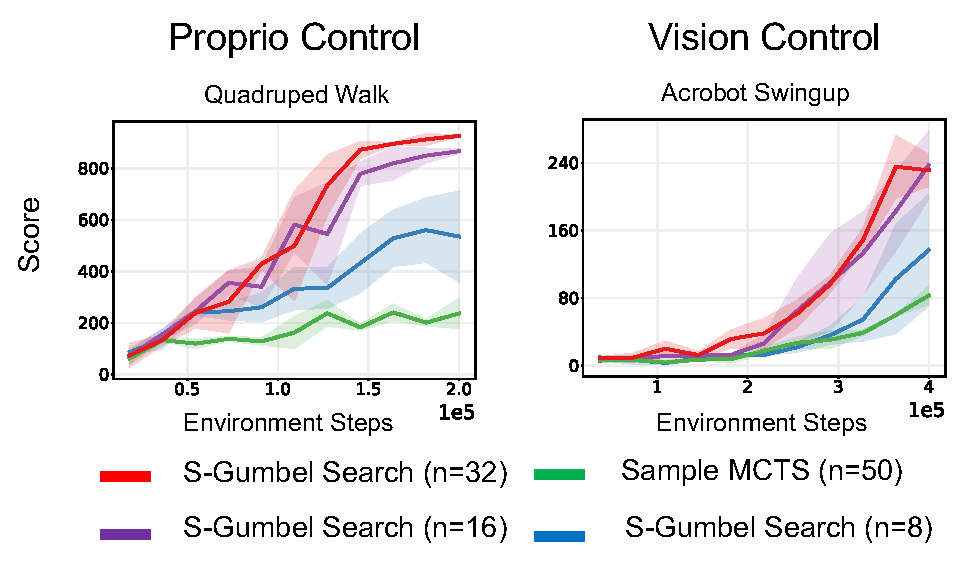
\includegraphics[width=0.45\textwidth]{sections/figs/ablation_search_main.pdf}
\caption{
Ablation study of our search method, namely the sampling-based Gumbel search (S-Gumbel search). We compare it with our search method with different numbers of simulations (n=16, 8) and Sample MCTS \citep{hubert2021learning}. Our method outperforms Sample MCTS, and increasing the number of simulations improves our method's performance on hard tasks.}
\label{ablation_search_main}
\end{figure}


\begin{figure}[t]
\centering
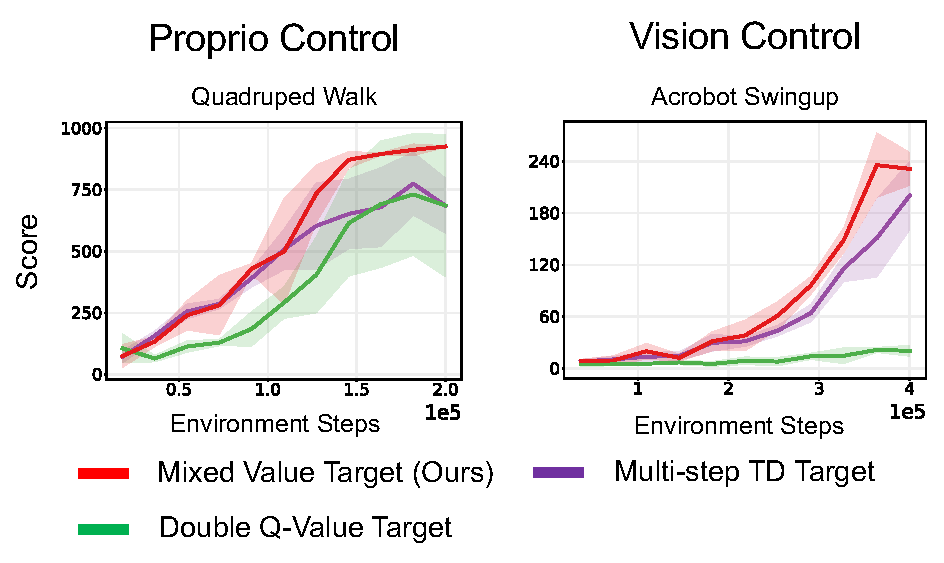
\includegraphics[width=0.45\textwidth]{sections/figs/ablation_value_main.pdf}
\caption{
Ablation study of our value target, known as the mixed value target. We compare it with different value targets, including the multi-step TD target and the double Q-value target. The mixed value target consistently achieves high performance in both Proprio Control and Vision Control tasks.}
\label{ablation_value_main}
\vspace{-10pt}
\end{figure}
\vspace{-5pt}

% adjusting the number of sampled actions from 8 to 4 to match the different simulation counts.
% The sampling-based Gumbel search and the mixed target value are the main algorithmic modifications we propose for EZ-V2.
% First, we compare the sampling-based Gumbel search method with the previous search method. Besides, we demonstrate that mixed value plays an important role in sample efficiency. 
% In this section, we discuss the effectiveness of the main modifications, the sampling-based Gumbel search and the mixed value target.

% \textbf{Ablations of Search}. The comparisons between our search and Sample MCTS are shown in Fig. \ref{ablation_search_main}. 
% Sample MCTS is a tree search method suitable for continuous control, which is proposed by Sample MuZero \citep{hubert2021learning}.
% In contrast to Sample MCTS (colored green), our search method (colored red) facilitates the algorithm to achieve better performance. 
% The Sample MCTS costs $n = 50$ simulations, while our method reduces the computation with only 32 simulations.

% We also plot the curves with 16 and 8 simulations. The number of sampled actions also varies from 8 to 4, matching different simulations. As we can see in Fig. \ref{ablation_search_main}, more simulations are beneficial in hard tasks like `Quadruped Walk', and our search method with 8 simulations can still beat Sample MCTS. 
% It illustrates the sampling-based Gumbel search keeps a better balance between exploration and exploitation due to the guarantee of policy improvement.
% We also provide the results of some other tasks in Fig. \ref{ablation_search}.
% Thus, we select 32 simulations as a sensible choice for our method.

\textbf{Ablations of Value Targets}. 
% The improved target value plays an important role in sample efficiency. 
% Since the benchmarks contain limited environment steps, it is essential to efficiently utilize the stale data from the replayed buffer. 
% Specifically, the value target is the sum of the predicted reward and the discount value of the predicted next state under the current policy. 
It can be seen in Fig. \ref{ablation_value_main} that our method (colored red) alleviates the off-policy issue compared with the multi-step TD target (colored purple), thus achieving better performance. Furthermore, we also compare with the value target 
$z_t$ derived from the optimal-Q Bellman equation, shown as follows:
\begin{equation}
    z_t = u_t + \gamma q(s_{t+1},a_{t+1}), \ \ a_{t+1} \sim p_t(a|s_{t+1})
\end{equation}
This technique also addresses the off-policy issue as the value target is based on the optimal Q-value estimation. Meanwhile, we employ the double Q-head trick. This estimation method is denoted as double Q-value target in Fig. \ref{ablation_value_main}.
Although the double Q-value target (colored green) also avoids the off-policy issue, the experiments illustrate that our method (colored red) exhibits consistent and robust performance across tasks. 
This is because our method matches the true value more rapidly by utilizing multi-step predicted rewards during the tree search.
Additional curves related to value ablation experiments can be found in Appendix \ref{ablation}.


Furthermore, practical comparisons between the TD-MPC2 and EZ-V2 algorithms in terms of computational load are provided in Appendix \ref{load}.



% Furthermore, EfficientZero V2 without the action embedding behaves with poor performance on some tasks, such as XX. The results indicate that the action embedding is moderately important for the learning of dynamic function due to the latent representation of the raw action. 


% \begin{figure*}[t]
% \centering
% 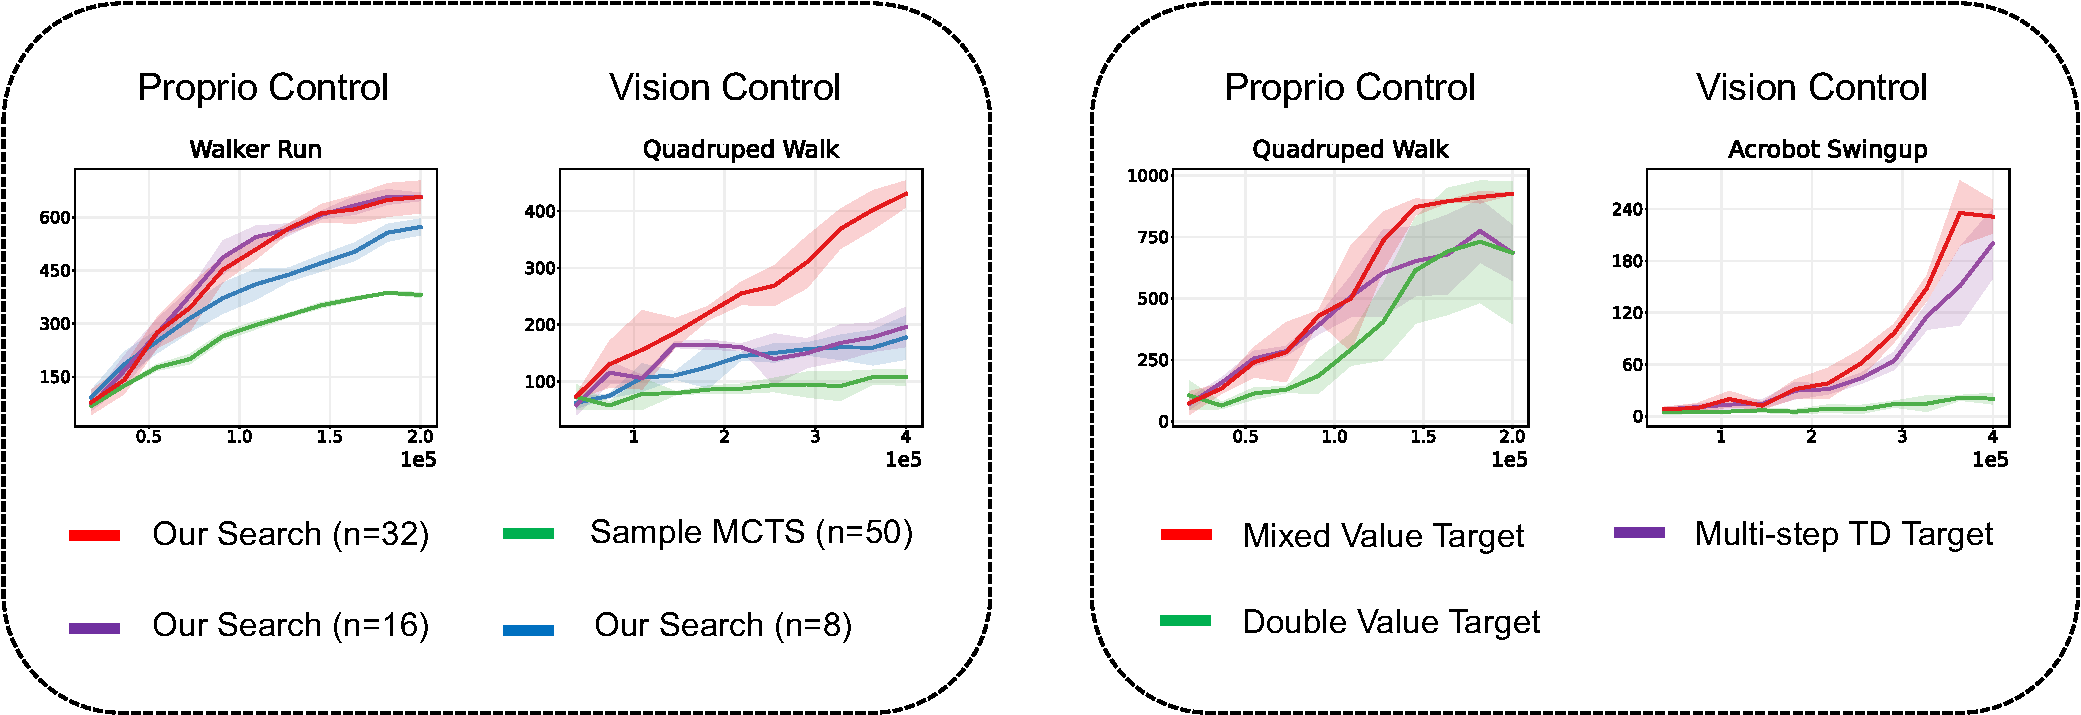
\includegraphics[width=0.8\textwidth]{sections/figs/ablation_main.pdf}
% \caption{Comparison between EfficientZero V2 and Dreamer V3. \ywr{More baselines?} We evaluate them under the Atari 100k, Proprio Control 100k, and Vision Control 200k benchmarks. For each metric, we obtain the normalized score from all environments that satisfies the corresponding settings.}
% \label{exp}
% \end{figure*}